%! Author = tulchin
%! Date = 15.02.2023

% Preamble
\documentclass[11pt]{article}
\usepackage[utf8x]{inputenc}
\usepackage[english,russian]{babel}
\usepackage{cmap}
\usepackage{graphicx}
\usepackage{gensymb}
\graphicspath{{./images/}}
\DeclareGraphicsExtensions{.pdf,.png,.jpg}

% Packages
\usepackage{amsmath}
\usepackage{amssymb}
\usepackage{amsfonts}
\usepackage{dsfont}
\usepackage[normalem]{ulem}
\usepackage{geometry}
\geometry{
    a4paper,
    top=25mm,
    right=15mm,
    bottom=25mm,
    left=15mm
}

% Document
\begin{document}

{\bf Задание 1}

    1) Мой браузер использует HTTP версии 1.1.
    На сервере используется HTTP тоже версии 1.1.

    2) Браузер может принимать языки: en, ru.
    Также передается информация о моем браузере, о моей системе.
    Можно узнать допустимое для клиента кодирование ответа.

    3) Адрес компьютера: 192.168.0.107.
    Адрес сервера: 128.119.245.12.

    4) Вернулось два кода: 200 для текста и 404 для картинки.

    5) Последнее изменение было в среду 15 февраля 2023 в 06:59:02 GMT.

    6) Контент вернулся размера 128 байт (для текста) + 209 байт (для ошибки загрузки картинки).

    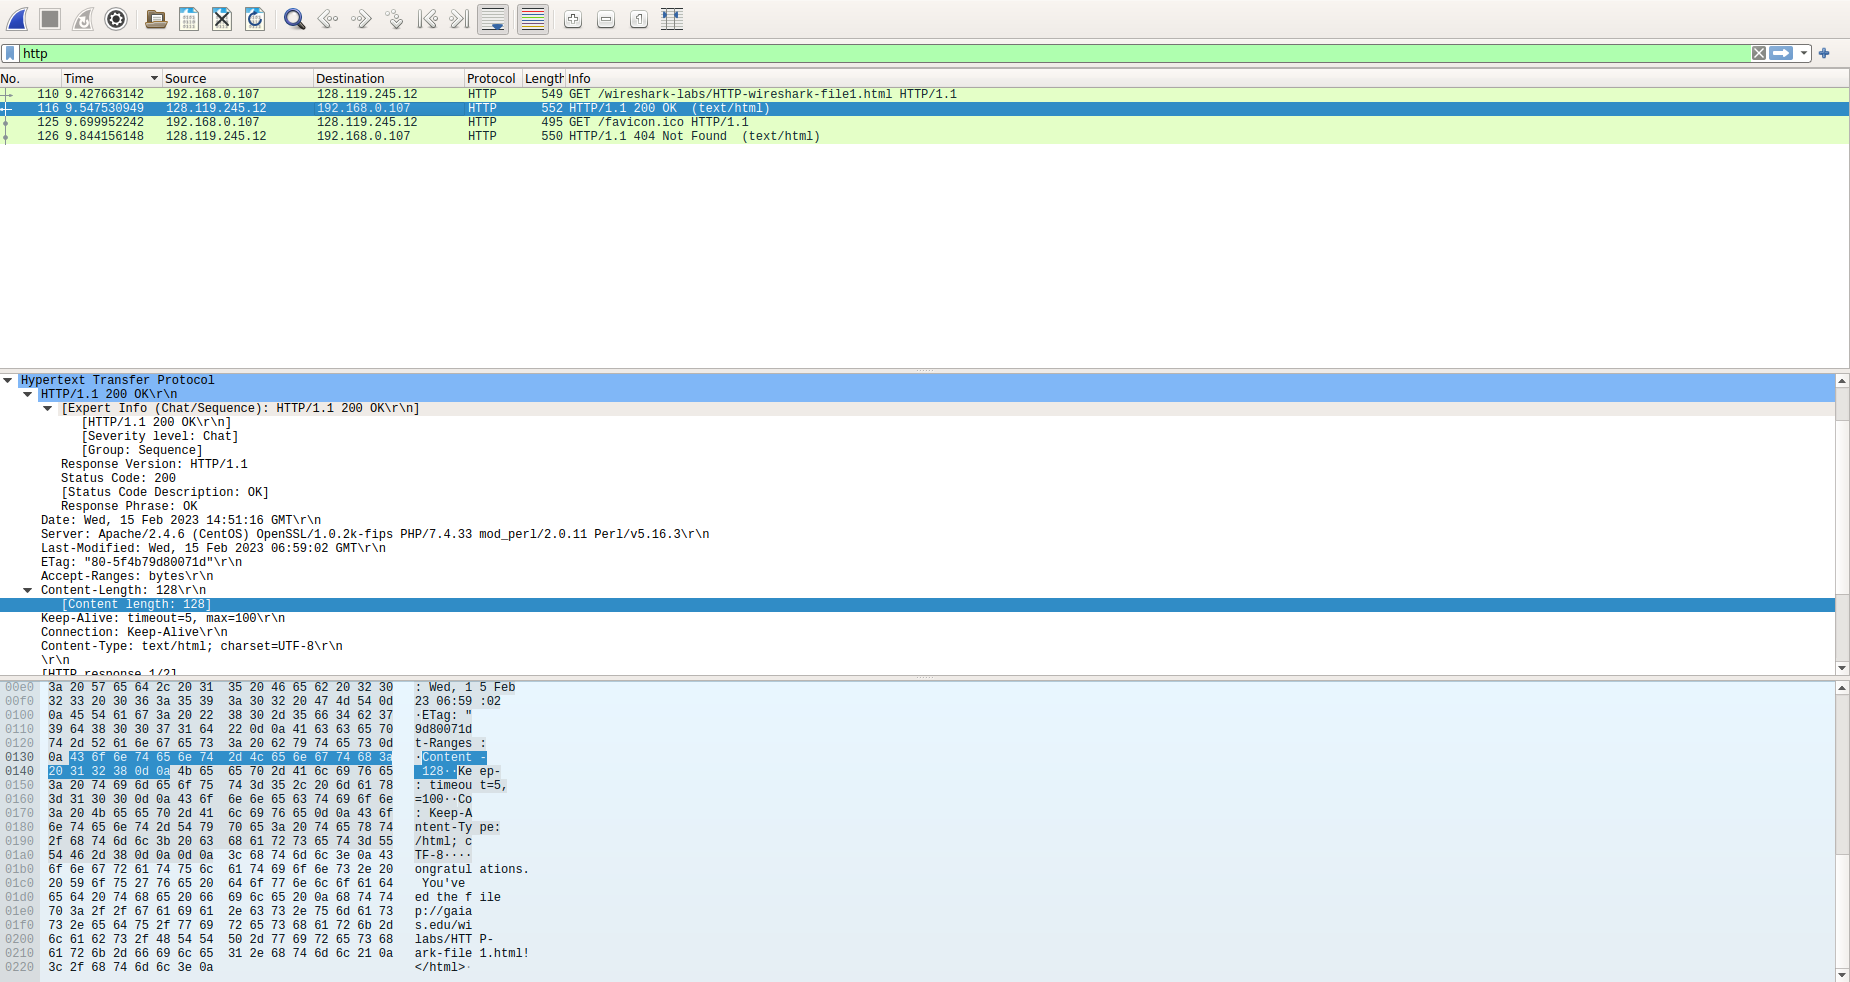
\includegraphics[width=\textwidth]{1.png}\\

    {\bf Задание 2}

    1) В первом GET запросе поля IF-MODIFIED-SINCE нет.

    2) Сервер вернул явно содержимое файла.
    Это можно увидеть ткнув на строку с ответом (код 200) и промотать его вниз.
    Там будет тело ответа.

    3) Да, во втором GET есть поле IF-MODIFIED-SINCE.
    Затем следует дата -- если данные были изменены после нее, то ответ будет с 200 кодом.
    Дата -- среда 15 февраля 2023, 06:59:02 GMT.

    4) Так как данные не были изменены после даты в IF-MODIFIED-SINCE поле, вернулся код 304.
    Сервер явно содержимое файлы не вернул.

    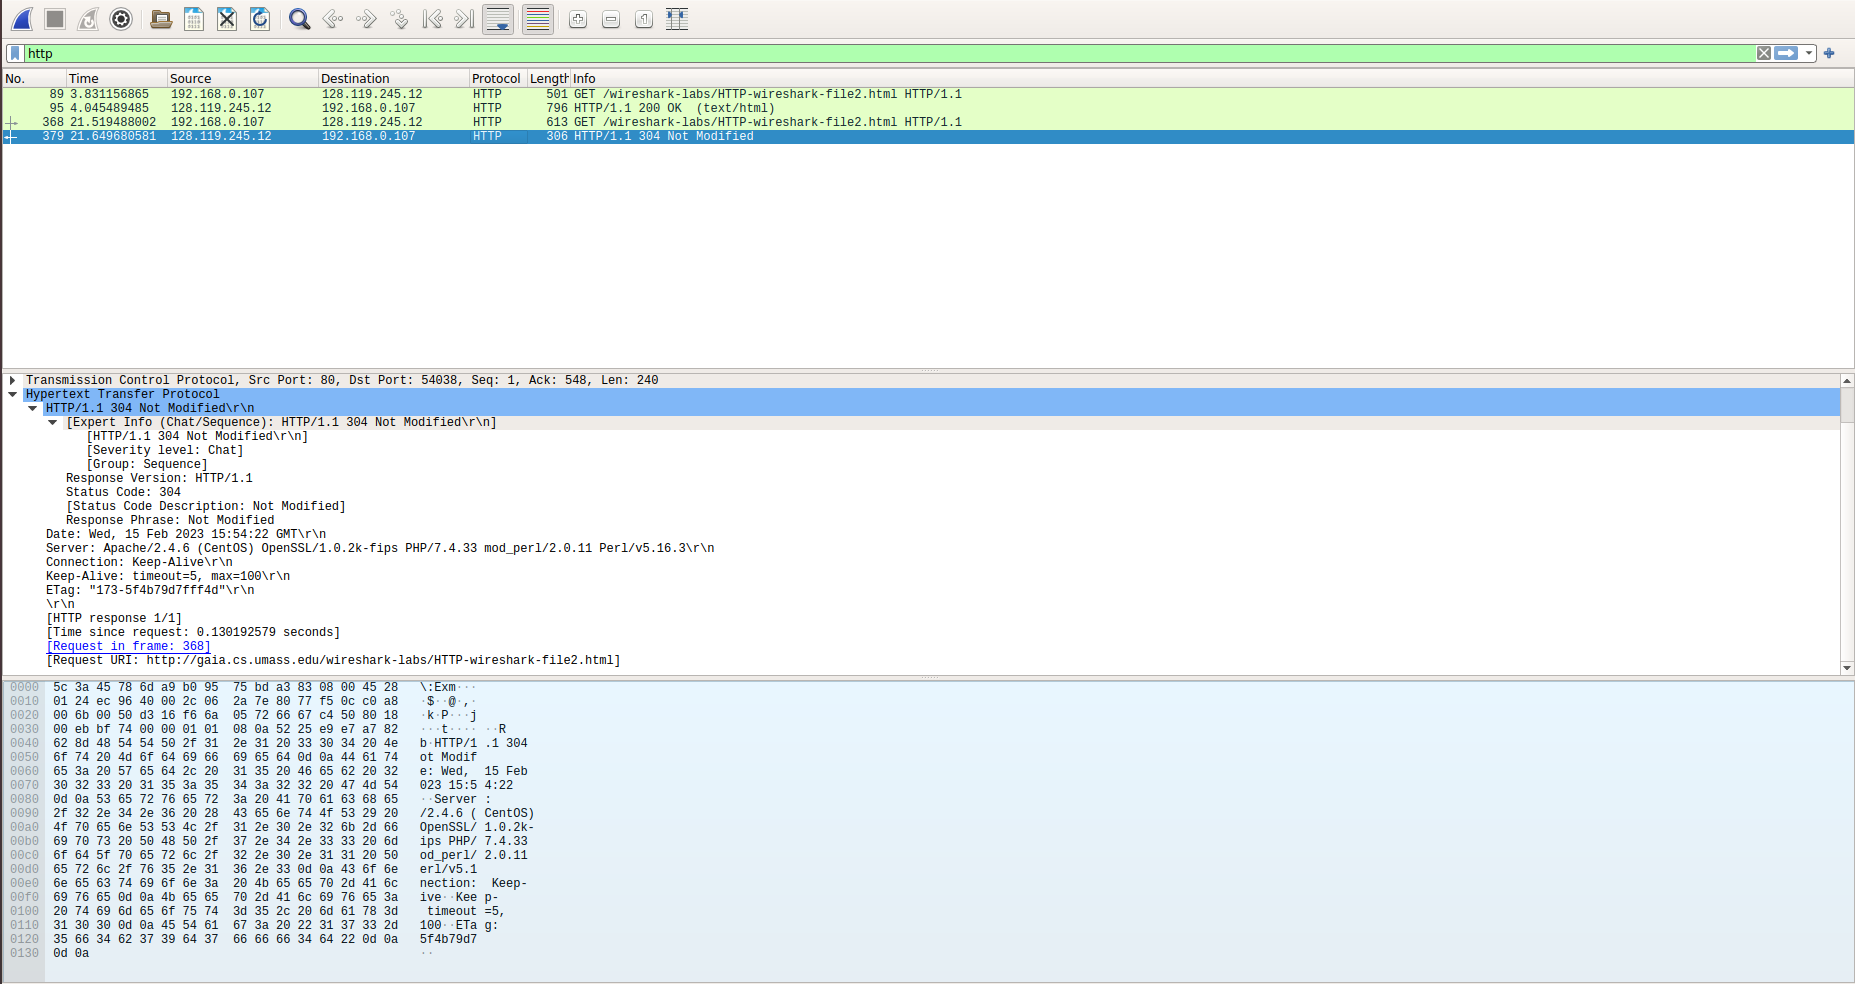
\includegraphics[width=\textwidth]{2.png}\\

    {\bf Задание 3}

    1) Всего был 1 запрос GET.
    Номер пакета 117.

    2) Вывод показал 3 сегмента с номерами 121, 123 и 125.

    3) 3 сегмента.

    4) В передаваемых данных можно найти количество сегментов, номер и размер каждого.

    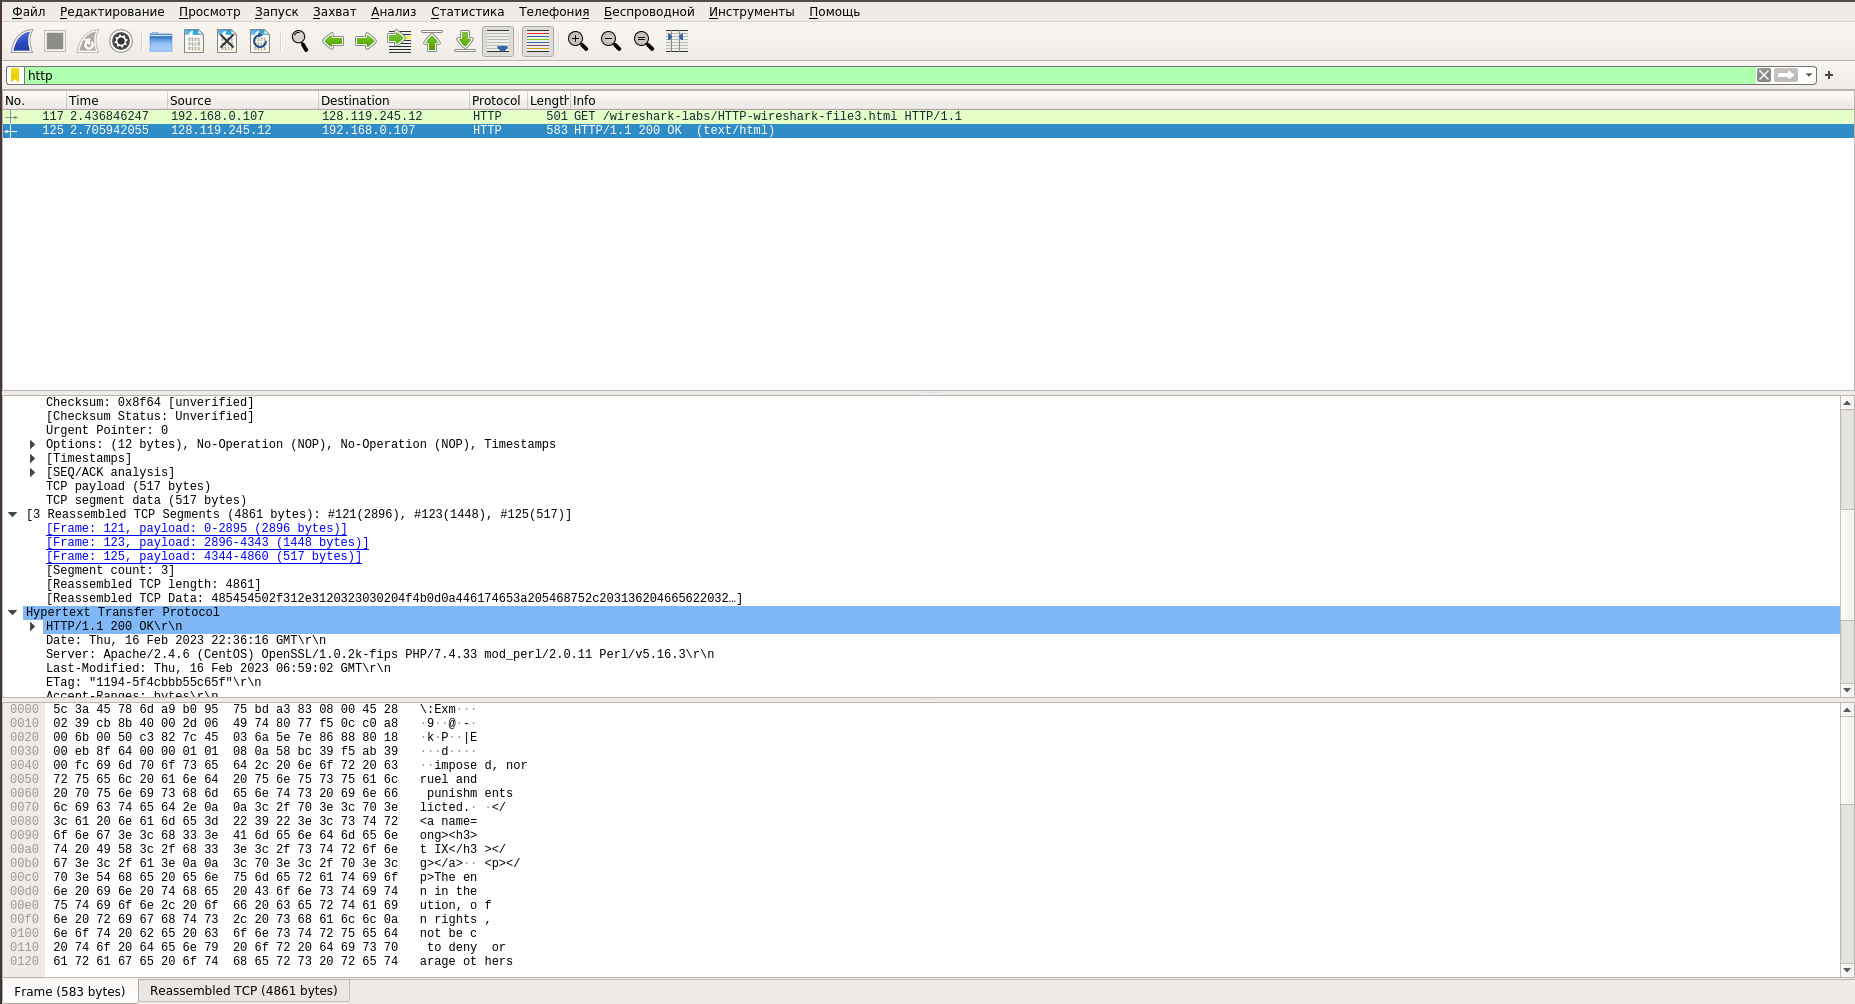
\includegraphics[width=\textwidth]{3.png}\\

    {\bf Задание 4}

    1) Было отправлено 3 GET запроса.
    Адреса: 128.119.245.12, 128.119.245.12, 178.79.137.164.

    2) Изображения были загружены параллельно.
    Если посмотреть на скриншот, то изображения были загружены в обратном порядке (относительно запросов).

    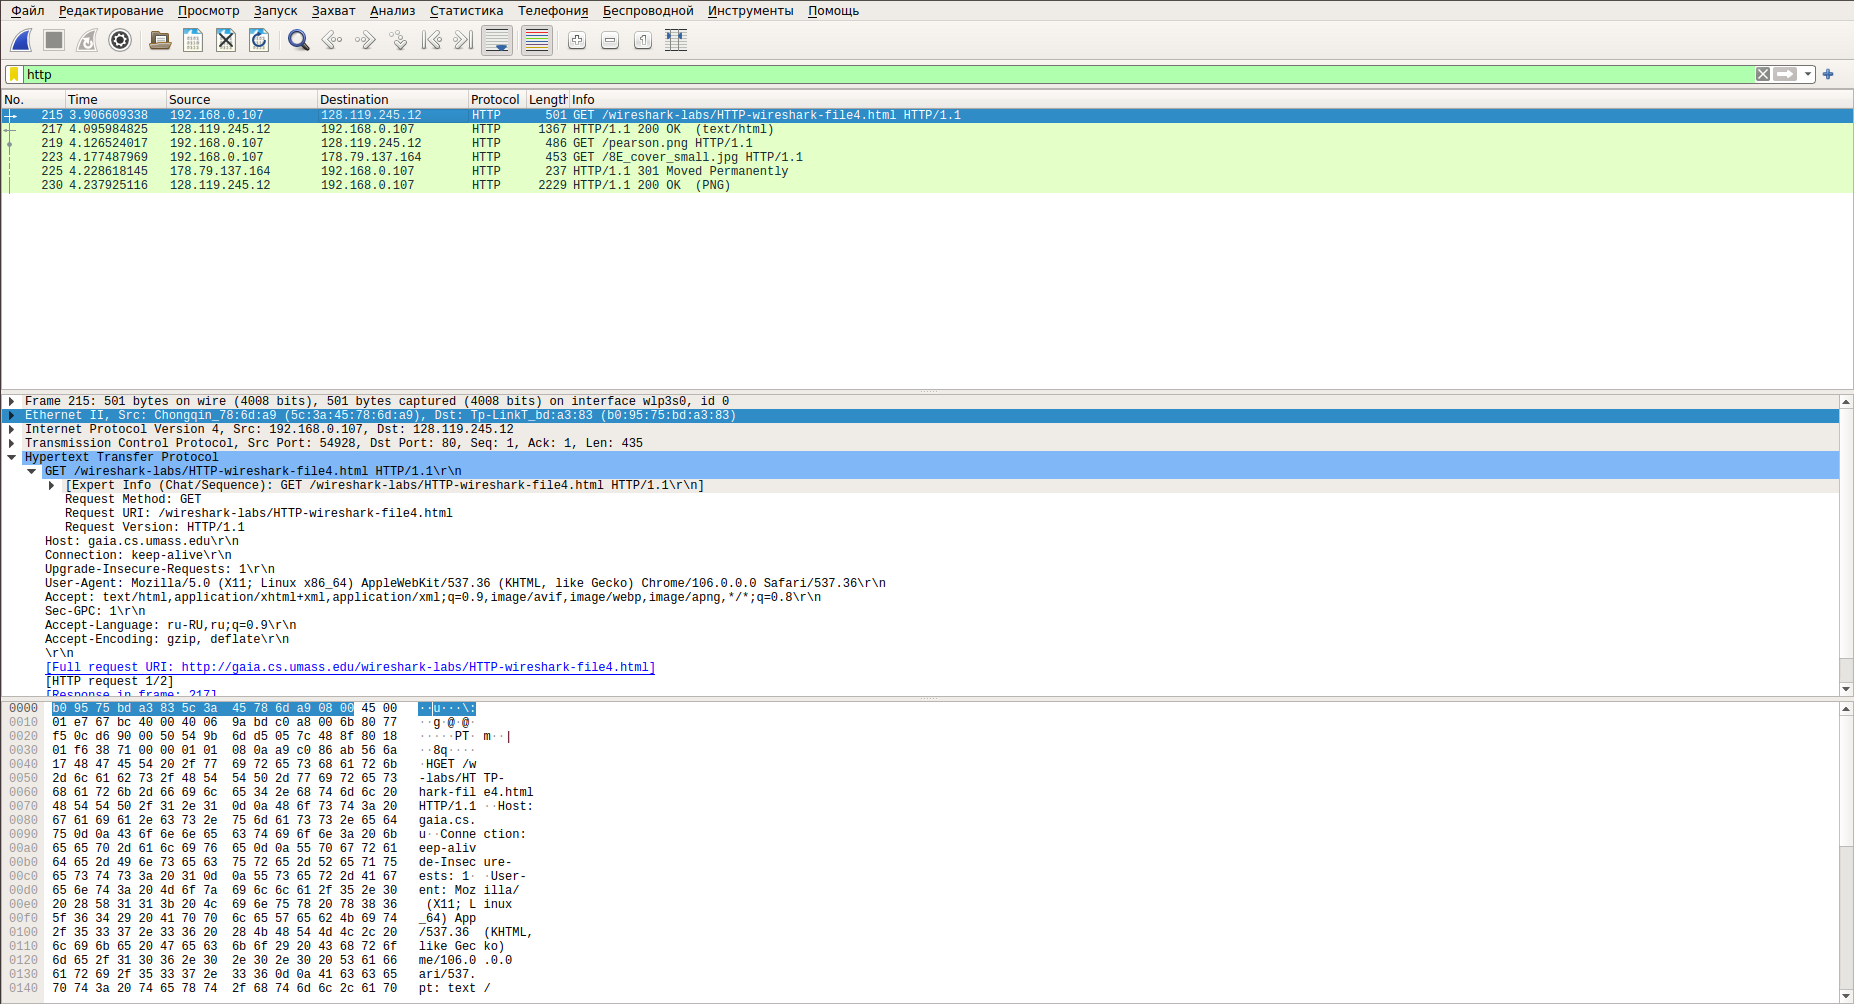
\includegraphics[width=\textwidth]{4.png}\\

    {\bf Задание 5}

    1) Ответ сервера: 401 Unauthorized.

    2) Во второй раз в запрос добавилось поле Authorization.
    Оно содержит логин и пароль, которые я ввел для доступа к сайту (Credentials).

    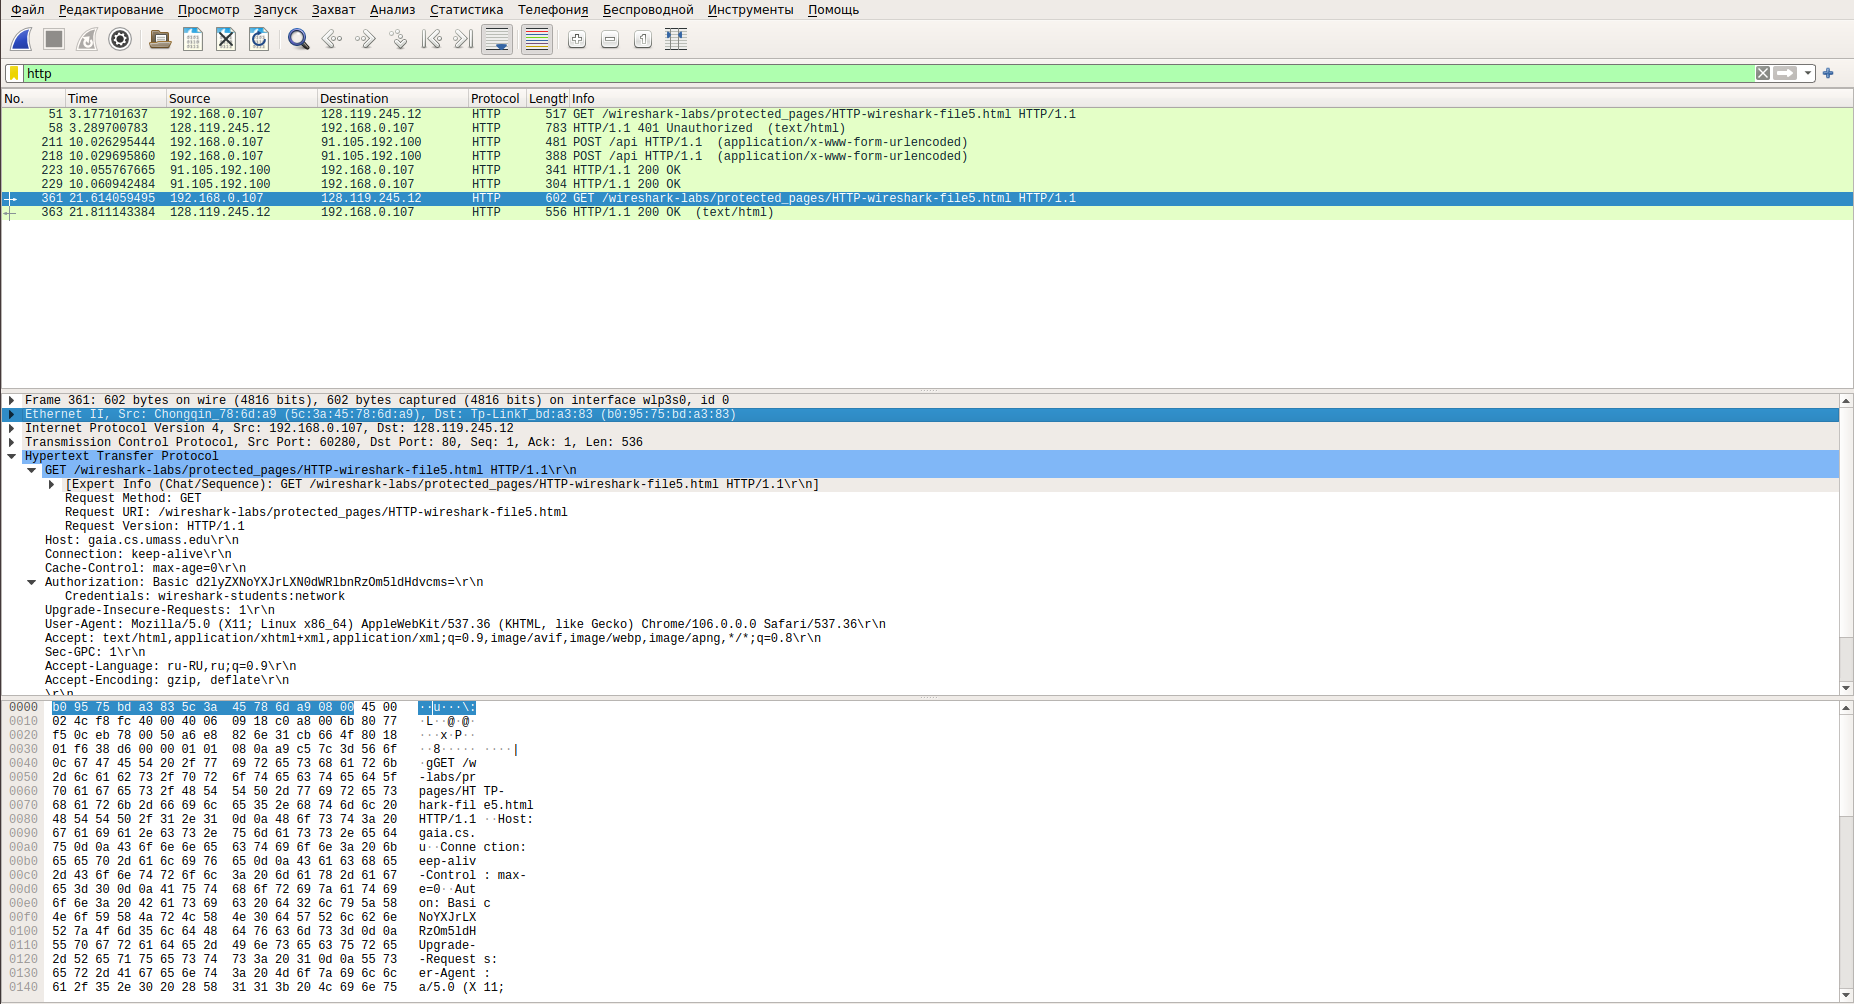
\includegraphics[width=\textwidth]{5.png}\\


\end{document}